\documentclass[11pt]{article}

\usepackage[pages=all, color=black, position={current page.south}, placement=bottom, scale=1, opacity=1, vshift=5mm]{background}
\SetBgContents{
	\tt This work is shared under a \href{https://creativecommons.org/licenses/by-sa/4.0/}{CC BY-SA 4.0 license} unless otherwise noted
}      % copyright

\usepackage[margin=1in]{geometry} % full-width

% AMS Packages
\usepackage{amsmath}
\usepackage{amsthm}
\usepackage{amssymb}
\usepackage{multirow}
% Unicode
\usepackage[utf8]{inputenc}
\usepackage{hyperref}
\hypersetup{
	unicode,
%	colorlinks,
%	breaklinks,
%	urlcolor=cyan, 
%	linkcolor=blue, 
	pdfauthor={Author One, Author Two, Author Three},
	pdftitle={A simple article template},
	pdfsubject={A simple article template},
	pdfkeywords={article, template, simple},
	pdfproducer={LaTeX},
	pdfcreator={pdflatex}
}

% Vietnamese
%\usepackage{vntex}

% Natbib
\usepackage[sort&compress,numbers,square]{natbib}
% \bibliographystyle{mplainnat}

% Theorem, Lemma, etc
\theoremstyle{plain}
\newtheorem{theorem}{Theorem}
\newtheorem{corollary}[theorem]{Corollary}
\newtheorem{lemma}[theorem]{Lemma}
\newtheorem{claim}{Claim}[theorem]
\newtheorem{axiom}[theorem]{Axiom}
\newtheorem{conjecture}[theorem]{Conjecture}
\newtheorem{fact}[theorem]{Fact}
\newtheorem{hypothesis}[theorem]{Hypothesis}
\newtheorem{assumption}[theorem]{Assumption}
\newtheorem{proposition}[theorem]{Proposition}
\newtheorem{criterion}[theorem]{Criterion}
\theoremstyle{definition}
\newtheorem{definition}[theorem]{Definition}
\newtheorem{example}[theorem]{Example}
\newtheorem{remark}[theorem]{Remark}
\newtheorem{problem}[theorem]{Problem}
\newtheorem{principle}[theorem]{Principle}

\usepackage{graphicx}
\graphicspath{{fig/}}

%\usepackage[linesnumbered,ruled,vlined,commentsnumbered]{algorithm2e} % use algorithm2e for typesetting algorithms
\usepackage{algorithm, algpseudocode} % use algorithm and algorithmicx for typesetting algorithms
\usepackage{mathrsfs} % for \mathscr command

\usepackage{lipsum}



\date{
\today
}

\begin{document}
% Author info
\title{Team 2}
%\author{Pradeep Atrey, Jonathan Muckell and Won Namgoong}
\author{Pradeep Atrey$^1$\thanks{Author One was partially supported by Grant XXX} \and Jonathan Muckell$^1$ \and Author Three$^2$\\
$^1$University at Albany, SUNY\\
$^2$New York University}
	\maketitle
	
\begin{abstract}
My abstract begins here... It starts with.... It is going to be a wondeful document.
		
% %		\noindent\textbf{Keywords:} article, template, simple
\end{abstract}

% % 	\tableofcontents

\section{Introduction}
\label{sec:intro}
These days, it is easy to find a capstone project \cite{Atrey2021BrickHouseSecuity}. It is easy to find a capstone project it is easy to find a capstone project it is easy to find a capstone project it is easy to find a capstone project it is easy to find a capstone project it is easy to find a capstone project it is easy to find a capstone project it is easy to find a capstone project it is easy to find a capstone project it is easy to find a capstone project it is easy to find a capstone project it is easy to find a capstone project it is easy to find a capstone project it is easy to find a capstone project it is easy to find a capstone project.

This is second para in introduction section....

\subsection{Preliminaries}\label{sec:prelim}
This is a subsection containing preliminaries.

\subsubsection{Notations}\label{sec:notations}
This is a subsection containing notations.

This is going to be my first equation (Eq. \ref{eqn:yofx}):
	
\begin{equation}\label{eqn:yofx}
 	y = f^{-1}_{z}(e^{\frac{2 \pi}{x}})    
\end{equation}
where, $x$ is a variable that does this, $z$ denotes \cite{Patil2019GeoSecureO}.

\section{Related Work}
\label{sec:relatedwork}
This section includes literature review.... As stated in Section \ref{sec:intro}, this is good.

These days, it is easy to find a capstone project....it is easy to find a capstone project it is easy to find a capstone project it is easy to find a capstone project it is easy to find a capstone project it is easy to find a capstone project it is easy to find a capstone project it is easy to find a capstone project it is easy to find a capstone project it is easy to find a capstone project it is easy to find a capstone project it is easy to find a capstone project it is easy to find a capstone project it is easy to find a capstone project it is easy to find a capstone project it is easy to find a capstone project.

These days, it is easy to find a capstone project....it is easy to find a capstone project it is easy to find a capstone project it is easy to find a capstone project it is easy to find a capstone project it is easy to find a capstone project it is easy to find a capstone project it is easy to find a capstone project it is easy to find a capstone project it is easy to find a capstone project it is easy to find a capstone project it is easy to find a capstone project it is easy to find a capstone project it is easy to find a capstone project it is easy to find a capstone project it is easy to find a capstone project.

%as shown in Figure \ref{fig:peer_exit}.

\section{Proposed Work}
\label{sec:proposedwork}
This section includes literature review.... As stated in Section \ref{sec:intro}, this is good.

\begin{equation}\label{eqn:ydash}
 	\mathcal{P} = \prod_{i=1}^{n}(\sum_{j=1}^{m}\frac{(p_i - p_j)^2}{(\sqrt{p_i} + \sqrt{p_j})^2})  
\end{equation}

As shown in Figure \ref{fig:peer_exit}, these days, it is easy to find a capstone project....it is easy to find a capstone project it is easy to find a capstone project it is easy to find a capstone project it is easy to find a capstone project it is easy to find a capstone project it is easy to find a capstone project it is easy to find a capstone project it is easy to find a capstone project it is easy to find a capstone project it is easy to find a capstone project it is easy to find a capstone project it is easy to find a capstone project it is easy to find a capstone project it is easy to find a capstone project it is easy to find a capstone project.

% 	\begin{figure}
% 		\centering
% 		
\includegraphics[width=0.5\textwidth]{example}
% 		\caption{This is my figure}
% 		\label{fig:peer_exit}
% 	\end{figure}
	
These days, it is easy to find a capstone project....it is easy to find a capstone project it is easy to find a capstone project it is easy to find a capstone project it is easy to find a capstone project it is easy to find a capstone project it is easy to find a capstone project it is easy to find a capstone project it is easy to find a capstone project it is easy to find a capstone project it is easy to find a capstone project it is easy to find a capstone project it is easy to find a capstone project it is easy to find a capstone project it is easy to find a capstone project it is easy to find a capstone project.

These days, it is easy to find a capstone project....it is easy to find a capstone project it is easy to find a capstone project it is easy to find a capstone project it is easy to find a capstone project it is easy to find a capstone project it is easy to find a capstone project it is easy to find a capstone project it is easy to find a capstone project it is easy to find a capstone project it is easy to find a capstone project it is easy to find a capstone project it is easy to find a capstone project it is easy to find a capstone project it is easy to find a capstone project it is easy to find a capstone project.

The following are the key contributions:
\begin{itemize}
    \item We designed the app.
    \item The accuracy is found as follows:
    \begin{enumerate}
        \item For FakeNewsNet dataset, it is 80\%.
        \item For MyOwn dataset, it is 85\%.
    \end{enumerate}
\end{itemize}

\begin{description}
    \item[Short] This is a shorter item label, and some text that talks
        about it. The text is wrapped into a paragraph, with successive
        lines indented.
    \item[Rather longer label] This is a longer item label.  As you can
        see, the text is not started a specified distance in -- unlike
        with other lists -- but is spaced a fixed distance from the end
        of the label.
\end{description}

These days, it is easy to find a capstone project....it is easy to find a capstone project it is easy to find a capstone project it is easy to find a capstone project it is easy to find a capstone project it is easy to find a capstone project it is easy to find a capstone project it is easy to find a capstone project it is easy to find a capstone project it is easy to find a capstone project it is easy to find a capstone project it is easy to find a capstone project it is easy to find a capstone project it is easy to find a capstone project it is easy to find a capstone project it is easy to find a capstone project.

\begin{figure}
\centering
            %  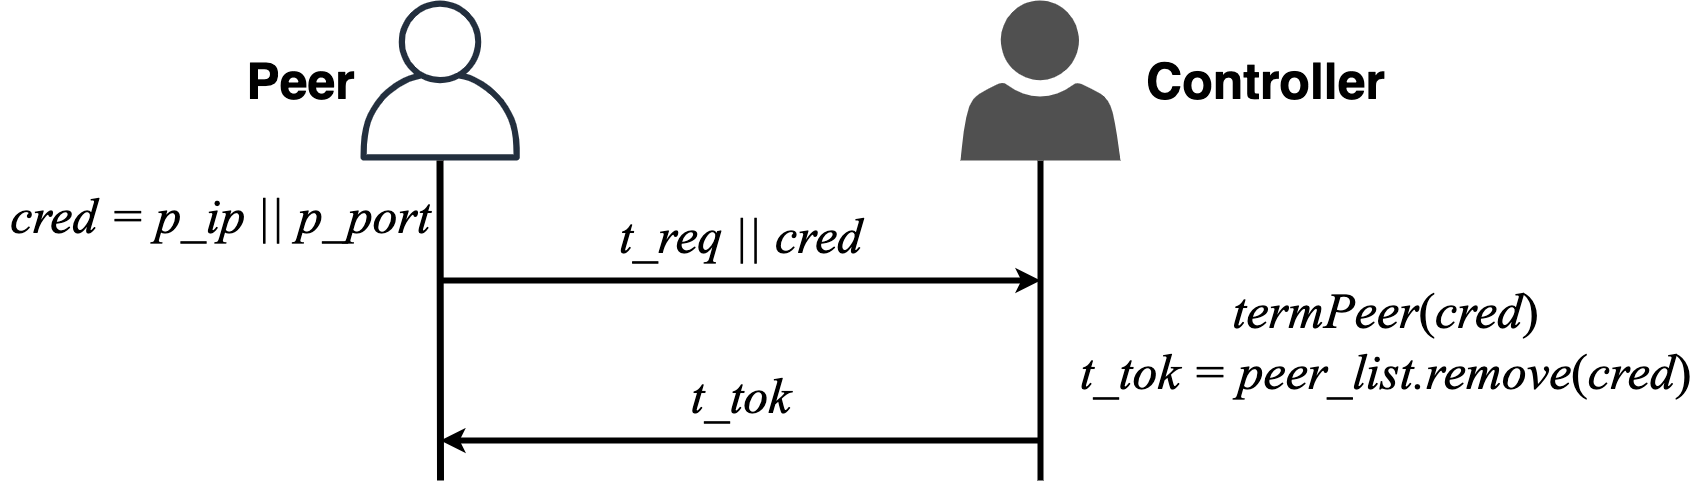
\includegraphics[width=0.7\textwidth]{Peer_Exit}
            %  \caption{This is Peer Exit figure}\label{fig:peer_exit}

        \begin{minipage}[b]{0.45\textwidth}
            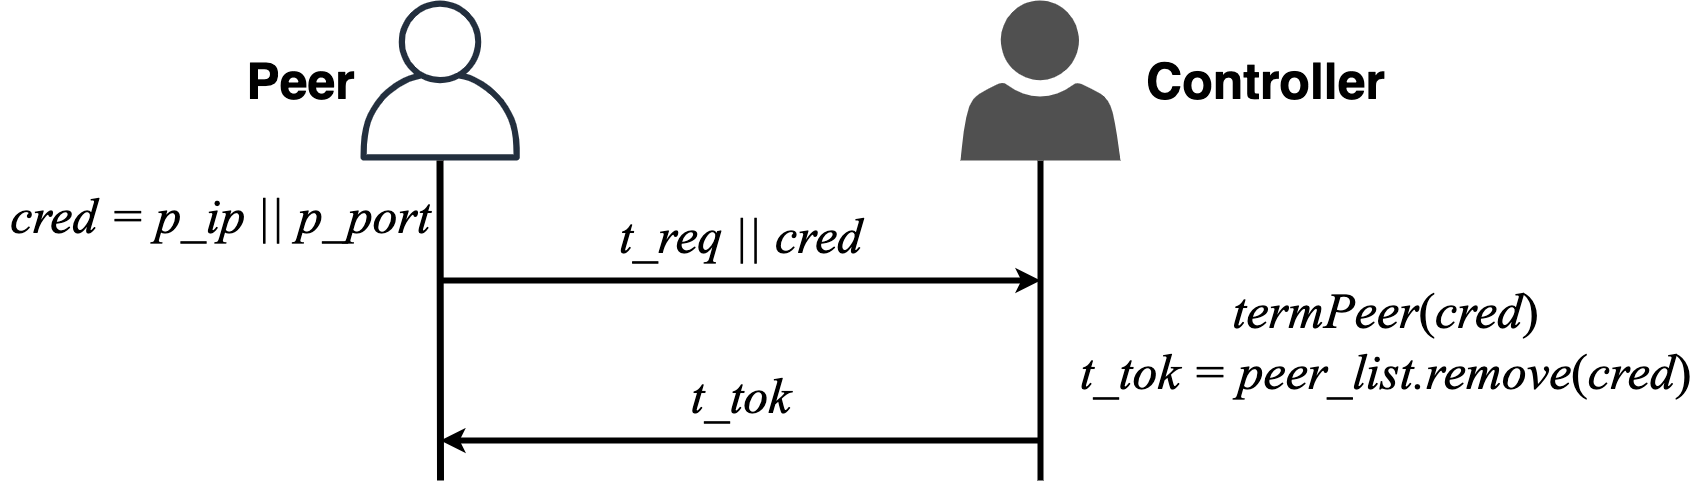
\includegraphics[width=0.9\textwidth]{Peer_Exit}
            \caption{This is Peer Exit figure}\label{fig:peer_exit}
        \end{minipage}
        \hfill
        \begin{minipage}[b]{0.45\textwidth}
            
\includegraphics[width=0.5\textwidth]{example}
            \caption{This is example figure}\label{fig:example}
        \end{minipage}
\end{figure}


	
% 	Second paragraph of introduction starts here...\cite{Rosen2011DisMaths}. 

% 	\subsection{Background}
% 	\label{sec:background}
% 	This subsection is for background....\cite{Berge1957GraphTheo} 	This subsection is for background.... 	This subsection is for background.... 	This subsection is for background.... 	This subsection is for background.... 	This subsection is for background.... 	This subsection is for background.... 	This subsection is for background.... 	This subsection is for background.... 	This subsection is for background.... 	This subsection is for background.... 	This subsection is for background.... 	This subsection is for background.... 	This subsection is for background.... 	This subsection is for background.... 	This subsection is for background.... 	This subsection is for background.... 	This subsection is for background.... 	This subsection is for background.... \cite{Patil2019GeoSecureO, Atrey2021BrickHouseSecuity}.

	
\begin{table}
\centering
\caption{This is my new table}
\label{tbl:new_table}
\begin{tabular}{|l|c|c|}
			\hline
 			\textbf{Number} & \textit{Odd} & \textit{Even$^*$} \\
			\hline \hline
 			1 & 4 & 6 \\ \hline
 			2 & 13 & 22 \\
% 			\multirow{2}{*}{1 and 2}&10.05 & Two \\ 
% 			 & 0.05 & Four \\
			\hline
\end{tabular}
\\$^*$ represents the even numbers
\end{table}
	
% 	This subsection is for background.... 	This subsection is for background.... 	This subsection is for background.... 	This subsection is for background.... 	This subsection is for background.... The following are the contributions in this work:
% 	\begin{itemize}
% 	    \item We do this....
% 	    \item And, this...
% 	\end{itemize}
	
% 	Further, the following are the key ideas in this work:
% 	\begin{enumerate}
% 	    \item The first key idea is to....
% 	    \item And, the second is... Moreover, it has the following two parts:
% 	    \begin{enumerate}
% 	        \item Number one.
% 	        \item Number 2.
% 	    \end{enumerate}
% 	\end{enumerate}

% 	Further, the following are the key ideas in this work:
% 	\begin{description}
% 	    \item [First] The first key idea is to....
% 	    \item [Second] And, the second is... 
% 	\end{description}

\begin{theorem}\label{thm_csp}
The proposed framework is secure against unauthorized reads from semi-malicious entities.
\end{theorem}
\begin{proof}
According to the assumptions stated above, the CSP is a semi-malicious entity. The CSP possesses read.
\end{proof}
% 	\subsection{Preliminaries}
% 	\label{sec:pre}
% 	This subsection is devoted to preliminaries.
	
% 	\subsubsection{Notations}\label{sec:notation}

% 	This is going to be my first equation:
	
% 	\begin{equation}\label{eqn:first_equation}
% 	y = f^{-1}_{z}(e^{\frac{2\pi}{x}})    
% 	\end{equation}
	
% 	As per equation \ref{eqn:first_equation}, $y$ is a function of $x$.
% 	\begin{equation}\label{eqn:second_equation}
% 	y = \sum_{i=1}^{n}{\sqrt{(x_i - 5)^2 - C}}  + \prod_{i=1}^{n-1}{(-\pi \times x_i)}
% 	\end{equation}
	
% 	\subsection{Previous Results}
% 	\label{sec:prev-results}
%     As discussed in section \ref{sec:pre}, ....
    
% 	Null graphs are discussed in \cite{HararyR74}
% 	The concept of ``internally stable set'' was used in \cite{Berge57, Berge58}.
	
% 	\begin{theorem}
% 		\label{thrm:1}
%         Given $y = x$, $z = y \times x$.
% 	\end{theorem}
% 	\begin{proof}
% 		We show that it is....
% 	\end{proof}

% 	\begin{corollary}
% 	\label{cor:1}
	
% 	\lipsum[5]
% 	\end{corollary}

% 	Unordered List (taken from Overleaf)
% 	\begin{itemize}
% 		\item The individual entries are indicated with a black dot, a so-called bullet.
% 		\item The text in the entries may be of any length.
% 	\end{itemize}

% 	Ordered List (taken from Overleaf)
% 	\begin{enumerate}
% 		\item The labels consists of sequential numbers.
% 		\item The numbers starts at 1 with every call to the enumerate environment.
% 	\end{enumerate}

	\begin{table}[ht]
		\centering
		\caption{This is a table}
		\label{tbl:1}
		\begin{tabular}{|c|c|}
			\hline
			\textbf{Odd} & \textbf{Even} \\
			\hline\hline
			One & Two \\
			\hline
			Three & Four \\
			\hline
		\end{tabular}

	\end{table}
	
\begin{table}[htbp]
\centering
\begin{tabular}{|c|c|c|c|p{1cm}p{1cm}p{1cm}p{1cm}p{1cm}p{1cm}p{1cm}|}
\hline
A & B & C & D & \multicolumn{7}{|c|}{F}  \\ \hline
\multirow{ 2}{*}{1} & 0 & 6 & 230 & 35 & 40 & 55 & 25 & 40 & 35 & \\
& 1 & 5 & 195 & 25 & 50 & 35 & 40 & 45 &  &  \\ \hline
\end{tabular}
\caption{A test caption}
\label{table2}
\end{table}

% 	Table~\ref*{tbl:1} is an example of a table.
	
% 	\section{More Examples}
% 	\label{sec:examples}
	
% 	Now we include a figure.
% 	(See Figure~\ref{fig:example}.)
% 	\begin{figure}[ht]
% 		\centering
% 		
\includegraphics[width=0.3\textwidth]{example}
% 		\caption{An example of a figure}
% 		\label{fig:example}
% 	\end{figure}
	
% 	\paragraph{Acknowledgements} \lipsum[6]
	
%	\newpage
    \bibliographystyle{IEEEtran}
	\bibliography{refs}
	
\appendix
	
\section{Omitted Proof in Section~\ref{sec:intro}}
	\label{app:1}
	dhjskahdlkashflks
% 	\lipsum[7]
	
\end{document}